% Dokumentenklasse (festgelegt!)
\documentclass{llncs}

% Allgemeine Einstellungen
\usepackage[utf8]{inputenc} % Zeichenkodierung auf UTF8
\usepackage[ngerman]{babel} % Deutsche Anpassungen, z.B. Trennregeln
\usepackage[T1]{fontenc} % T1-Zeichenkodierung einschalten, damit z.B. Umlaute im PDF-Dokument gesucht werden können

\usepackage[a4paper,top=3cm,bottom=2cm,left=3cm,right=3cm,marginparwidth=1.75cm]{geometry}

% Quellenverzeichnis:
\usepackage[backend=biber, style=numeric, sorting=none]{biblatex}
\addbibresource{Seminar_Quellenverzeichnis.bib}

% für TODO Kommentare:
\usepackage{todonotes}

% Quellcode-Abbildungen:
\usepackage{listings}

% Vektorgrafiken
\usepackage{svg}

% Tabellenbeschriftung
\usepackage{caption}
\captionsetup[table]{position=below,skip=1em}

% Farbe in Tabellenzellen:
\usepackage{colortbl}
\definecolor{hellgrau}{rgb}{0.95,0.95,0.95} % Farbdefinition, kann im Code verwendet werden

% Bilder einbinden:
\usepackage{graphics}
\graphicspath{{./img/}} % Angabe von Ordner für Bilder
\usepackage{subcaption}


\begin{document}
\title{Intertask Kommunikation in Echtzeitbetriebsystemen}
\author{Stefan Lindörfer\\
\email{stefan.lindoerfer@stud-mail.uni-wuerzburg.de}
}
\institute{
	Universität Würzburg\\
	Institut für Informatik\\
	Lehrstuhl V - Technische Informatik\\
	Seminar: Embedded Systems\\bei Prof. Dr. Reiner Kolla\\Wintersemester 2020/21}

%\date{}

\maketitle

\renewcommand{\abstractname}{Abstract}

\begin{abstract}
	Die Informationsübermittlung zwischen Tasks in Echtzeitbetriebssystemen ist von fundamentaler Bedeutung und kann je nach Anforderungsszenario auf verschiedene Arten erfolgen. In der vorliegenden Arbeit wird zunächst ein Überblick über die verschiedenen Möglichkeiten der Koordinierung und Synchronisierung von Tasks gegeben und gezeigt, wie Daten zwischen Tasks ausgetauscht werden können. Anschließend wird jeweils vertieft auf die einzelnen Mechaniken eingegangen und Implementierungsansätze aufgezeigt.
\end{abstract}

\section{Einführung}
\label{subsec:Einführung}
Echtzeitbetriebssysteme (auch \textbf{R}eal \textbf{T}ime \textbf{O}perating \textbf{S}ystems, kurz RTOS genannt) sind aus der Informatik nicht mehr wegzudenken und begegnen uns oft unbewusst im Alltag in zahlreich verschiedenen Anwendungsgebieten. So werden sie etwa in modernen Automobilen als Betriebssysteme eingesetzt, zur Steuerung und Regelung industrieller Anlagen verwendet oder im Verkehrswesen (z.B. Schienenverkehr- oder Ampelsteuerungen) genutzt \autocite[vgl.][157]{Winzker2008}. Auch als Betriebssysteme von Satelliten in der Raumfahrt sowie für den Einsatz in Flugzeugen sind sie geeignet \autocite{Wuerzburg2019}.\\

Die Besonderheit dieser Art von Betriebssystemen ist die Fähigkeit, Echtzeit-Anforderungen umsetzen zu können. Das bedeutet (anders als bei Nicht-RTOS) als Softwareentwickler die Zusicherung seitens des Betriebssystems zu besitzen, dass eine bestimmte Aufgabe innerhalb eines vordefinierten Zeitfensters entweder ausgeführt und ggf. abgeschlossen (oder unterbrochen) wird. Betriebssysteme anderer Kategorien führen ihre Aufgaben meist schnellstmöglich bzw. ohne Vorhersagemöglichkeit aus und passen kein Zeitfenster ab, garantieren also keine Echtzeit, sondern setzen auf größtmögliche Performanz \autocite[vgl.][317]{HeinzWoern2005}.\\

Aufgaben in Echtzeitbetriebssystemen sind in sogenannte Tasks (oder auch Threads) unterteilt, die vom Betriebssystem getrennt voneinander verwaltet werden. Abhängig vom jeweiligen Szenario können Tasks jedoch nicht ausschließlich getrennt voneinander operieren und ihren jeweiligen Aufgaben nachgehen, sondern ein Informationsaustausch zwischen ihnen ist erforderlich: Um etwa einen Ablauf abzubilden, bei dem zuerst Task A und anschließend Task B ausgeführt werden soll, muss zunächst eine Information von A nach B übermittelt werden können, die den entsprechenden Prozessfortschritt anzeigt, sodass B beginnen kann. Oder auch wenn Daten eines Tasks von einem anderen zur (synchronisierten) Weiterverarbeitung benötigt werden, ist ein entsprechender Kommunikationskanal erforderlich um die Daten zu transferieren.\\

Dieser gesamte interne Informationsaustausch wird als Intertask-Kommunikation bezeichnet. Es existieren mehrere allgemeine Möglichkeiten und Techniken, Informationen und Daten zwischen Tasks auszutauschen, abhängig vom jeweiligen Szenario und den Anwendungsanforderungen. Diese Techniken werden im Folgenden aufgezeigt und nacheinander erläutert.

\subsection{Überblick}
\label{subsec:Überblick}
Grundsätzlich unterteilt man Intertask-Kommunikation in drei Kategorien \autocite[vgl.][79]{Cooling2017}:
\begin{enumerate}
	\setlength\itemsep{0.5em} % Zeilenabstand der Punkte ändern
	\item \textbf{Synchronisation und Koordination von Tasks ohne Datentransfer} \label{subsec:Überblick:Punkt1}
	\item \textbf{Datentransfer zwischen Tasks ohne Synchronisation} \label{subsec:Überblick:Punkt2}
	\item \textbf{Datentransfer zwischen Tasks mit Synchronisation} \label{subsec:Überblick:Punkt3}
\end{enumerate}
Punkt (\ref{subsec:Überblick:Punkt1}) enthält anders als (\ref{subsec:Überblick:Punkt2}) und (\ref{subsec:Überblick:Punkt3}) keinen Datentransfer und unterscheidet sich von diesen - wie bereits in Kapitel \ref{subsec:Einführung} ausgeführt - dadurch, dass lediglich eine Information ausgetauscht bzw. vom Empfänger abgefragt wird, um Tasks zu synchronisieren oder einen Arbeitsablauf umzusetzen. Während bei (\ref{subsec:Überblick:Punkt2}) und (\ref{subsec:Überblick:Punkt3}) ein Datentransfer insofern stattfindet, als das Daten ausgetauscht und vom Empfänger für die Weiterverarbeitung genutzt werden, sie also nicht zwingend für eine Ablaufsteuerung verwendet werden \autocite[vgl.][80]{Cooling2017}.

\subsection{Begriffsgrundlage}
\label{subsec:Begriffsgrundlage}
Für eine genauere Betrachtung der einzelnen Kategorien aus \ref{subsec:Überblick}, müssen zunächst die beiden Begriffe Koordination und Synchronisation definiert und pragmatisch voneinander abgegrenzt werden:
\begin{itemize}
	\setlength\itemsep{1em} % Zeilenabstand der Punkte ändern
	\item \textbf{Koordination}: \textit{\glqq Das Integrieren und Anpassen (einer Reihe von Teilen oder Prozessen), um eine reibungslose Beziehung zueinander herzustellen.\grqq} \autocite[80]{Cooling2017}
	\item \textbf{Synchronisation}: \textit{\glqq Etwas verursachen, bewegen oder ausführen, genau zur exakten Zeit.\grqq} \autocite[80]{Cooling2017}
\end{itemize}
Es fällt auf, dass die Definition der Koordination keinen Bezug zur Zeit beinhaltet. Der wesentliche Unterschied zwischen Koordinierung und Synchronisierung ist somit der Zeit-Faktor \autocite[vgl.][80]{Cooling2017}. Während mit einer Koordination ein theoretisch zeitunabhängiger, sequentieller Ablauf von Tasks angestrebt wird, meint Synchronisation dagegen das zeitliche Abgleichen von Vorgängen und legt damit verstärkt Fokus auf die Kerneigenschaft von Echtzeitbetriebssystemen. Dennoch haben beide Begriffe in dieser Thematik ihre klare Daseinsberechtigung und ihre bevorzugten Anwendungsbereiche in denen sie zum Tragen kommen.

\section{Task-Interaktion ohne Datentransfer}
\label{sub:Task_Interaktion_ohne_Datentransfer}
Müssen, wie schon in \ref{subsec:Überblick} erwähnt, keine Daten im eigentlichen Sinne zwischen Tasks transferiert werden, sondern nur ein Arbeitsablauf gesteuert werden, spricht man von Task-Interaktion ohne Datentransfer. Dies kann sowohl mit dem Ziel einer Task-Synchronisation durchgeführt werden als auch ohne den bereits festgestellten Zeit-Faktor mittels Koordination, siehe \ref{subsec:Begriffsgrundlage}. Demzufolge wird bei den Möglichkeiten dieser Kategorie auch in diese beiden Fälle unterschieden. Tabelle \ref{tab:Konstrukte} zeigt diese Unterscheidung auf und gibt gleichzeitig einen Überblick über die jeweils zu verwendeten Konstrukte dieser Kategorie.

\begin{table}
	\centering % Tabelle zentrieren
	\def\arraystretch{1.5} % Vertikales Padding
	\setlength{\tabcolsep}{0.5em} % Horizontales Padding
	\fbox{ % Rahmen um Tabelle
\begin{tabular}[h]{l|l|l}
	\textbf{Koordination} & \multicolumn{2}{c}{\textbf{Synchronisation}} \\
	\hline
	Condition Flags & Event Flags & Signale \\
	\hline
	\underline{\textit{Operationen:}} & \underline{\textit{Operationen:}} & \underline{\textit{Operationen:}} \\
	\texttt{Set} & \texttt{Set} & \texttt{Wait} \\
	\texttt{Clear} & \texttt{Clear} & \texttt{Send} \\
	\texttt{Check} & \texttt{Check} & \texttt{Check}
\end{tabular}}
\caption{\label{tab:Konstrukte} Koordinierungs- und Synchronisationskonstrukte \autocite[vgl.][82]{Cooling2017}}
\end{table}
Grundsätzlich ist ein Flag (Flagge) ein Statusindikator, der einen bestimmten Zustand anzeigt. Im simpelsten Fall sind das $0$ und $1$. Für das Ziel einer Koordination, werden sogenannte Condition Flags verwendet. Ist Synchronisierung erforderlich, dass also der gesteuerte Prozess zeitkritisch auszuführen ist, dann können - je nach Anwendungsfall - Event Flags oder Signale verwendet werden. Alle drei Konstrukte und deren Operationen werden im Folgenden detaillierter erläutert.

\subsection{Task-Koordinierung mit Condition Flags}
\label{subsec:Koordinierung_mit_Condition_Flags}
Die einfachste Möglichkeit der Koordination ist das Condition Flag. Tabelle \ref{tab:Konstrukte} zeigt die auf Condition Flags anwendbaren Operationen \texttt{Set} (setzen), \texttt{Clear} (zurücksetzen) und \texttt{Check} (überprüfen).

\begin{figure}[h]
\centering
\def\svgwidth{300pt}
%\def\svgwidth{\columnwidth} % Breite wird auf Blattbreite (spalte) gesetzt
\input{ConditionFlag.pdf_tex}
\caption{\label{fig:ConditionFlag} Einfache Benutzung von Condition Flags \autocite[vgl.][83]{Cooling2017}}
\end{figure}

Abbildung \ref{fig:ConditionFlag} zeigt exemplarisch, wie Condition Flags verwendet werden: Task A übernimmt in diesem Fall die Steuerung des Ablaufs, während Task B darauf wartet ausgeführt zu werden und fortlaufend in regelmäßigen Abständen überprüft (\texttt{Check}), ob das Flag gesetzt wurde. Im einfachsten Fall wird dafür eine globale Boolean-Variable eingesetzt, bei dieser $true$ den Zustand \texttt{Set} und $false$ den Zustand \texttt{Clear} repräsentieren kann. Ist es erforderlich mehrere Zustände einzusetzen, können Aufzählungstypen wie Enums verwendet werden. Diese bieten auch den Vorteil der besseren Lesbarkeit des Quellcodes, da sofort eindeutig ablesbar ist, welcher Flag-Zustand \texttt{Set} bzw. \texttt{Clear} darstellt. Für die meisten Anforderungen ist dieses Vorgehen der Implementierung von Condition Flags absolut ausreichend \autocite[vgl.][84]{Cooling2017}.\\

In kritischeren Situationen jedoch, z.B. bedingt durch hohe Zugriffsraten auf ein Flag (es können sich Lese- oder Schreibfehler ergeben) oder wenn ein höheres Maß an Ausfallsicherheit (keine Redundanz!) gewünscht ist, empfiehlt sich eine Mehrfachabsicherung wie sie Abbildung \ref{fig:ConditionFlag2} demonstriert:

\begin{figure} [h]
	\centering
	\def\svgwidth{300pt}
	%\def\svgwidth{\columnwidth} % Breite wird auf Blattbreite (spalte) gesetzt
	\input{ConditionFlagII.pdf_tex}
	\caption{\label{fig:ConditionFlag2} Verbesserte Benutzung von Condition Flags zur Koordination \autocite[vgl.][84]{Cooling2017}}
\end{figure}

Für jeden Zustand, der gesetzt werden kann (hier: Zwei), existiert jetzt ein eigenes Condition Flag. Task A übernimmt in diesem Fall ausschließlich das Setzen der Zustände, führt diese Operation jedoch nur durch, falls das entsprechende Flag vorher von Task B zurückgesetzt wurde \autocite[vgl.][85]{Cooling2017}. Task B prüft im Unterschied zur Abbildung \ref{fig:ConditionFlag} jetzt zusätzlich den Zustand aller relevanten Flags (bezogen auf Abbildung \ref{fig:ConditionFlag2} also beide) bevor auf einen \texttt{Set}-Zustand reagiert wird \autocite[vgl.][85]{Cooling2017}. Wenn Unstimmigkeiten auftreten, weil z.B. das Prüfergebnis keinen eindeutig definierten Gesamtzustand ausweist, kann ein Fehlverhalten rechtzeitig abgefangen werden. Anders als dies bei Abbildung \ref{fig:ConditionFlag} möglich ist, denn dort kann u.U. kein Fehlverhalten vom Empfänger-Task festgestellt werden, da keine Absicherungsinstanz existiert mit der verglichen werden kann. Nach einem erfolgreichem \texttt{Check} wird das ausgeführte Flag wieder von B zurückgesetzt. Umgesetzt wird dies wieder mittels Enums, wie folgender Codeabschnitt für Abbildung \ref{fig:ConditionFlag2} zeigt:
\begin{lstlisting}[language=C]
typedef enum {StartSet, StartClear} StartFlag;
typedef enum {StopSet, StopClear} StopFlag;
\end{lstlisting}
Diese Herangehensweise führt, wie bereits ausgeführt, zu einer sichereren und zuverlässigeren Abwicklung der Koordinierung und besitzt auch die bereits festgestellte Eigenschaft der besseren Lesbarkeit. An dieser Stelle sei noch erwähnt, dass eine Implementierung auf globaler Ebene ebenfalls Nachteile mit sich bringen kann (schlechtere Performanz, unkontrollierter Zugriff) und deswegen in objektorientierten Programmiersprachen eine Kapselung in einem separatem Objekt eine Möglichkeit ist, die bevorzugt werden sollte.\\

Eine weitere Möglichkeit der Organisation mit Condition Flags sind \textbf{Flag Gruppen}. Diese bieten sich besonders dann an, wenn viele Zustände abgebildet werden sollen, die zudem logisch miteinander in Verbindung stehen können. Wenn beispielsweise etwa in einem einfachen Fall Zustand A (Flag A) nicht gleichzeitig mit Zustand B (Flag B) aktiv sein darf. Dabei werden einzelne Flags auf Wortbreite zusammengefasst (auch eine geringere Breite ist möglich, z.B. durch Einsatz einer Variablen), in der jedes Bit ein Flag repräsentieren kann. Abbildung \ref{tab:FlagGroup} zeigt dieses Konzept auf einer 2 Byte Variablen mit je 8 Bits.\\
\begin{table}[h]
	\centering % Tabelle zentrieren
	\def\arraystretch{1.5} % Vertikales Padding
	\setlength{\tabcolsep}{0.5em} % Horizontales Padding
	%\fbox{ % Rahmen um Tabelle
		\begin{tabular}[h]{|l|c|c|c|c|c|c|c|c|c|c|c|c|c|c|c|c|}
			\hline
			\textbf{Bit} & \cellcolor{hellgrau}15 & \cellcolor{hellgrau}14 & \cellcolor{hellgrau}13 & \cellcolor{hellgrau}12 & \cellcolor{hellgrau}11 & \cellcolor{hellgrau}10 & \cellcolor{hellgrau}9 & \cellcolor{hellgrau}8 & \cellcolor{hellgrau}7 & \cellcolor{hellgrau}6 & \cellcolor{hellgrau}5 & \cellcolor{hellgrau}4 & \cellcolor{hellgrau}3 & \cellcolor{hellgrau}2 & \cellcolor{hellgrau}1 & \cellcolor{hellgrau}0 \\
			\hline
			\textbf{Wert} & 1 & 0 & 0 & 1 & 0 & 1 & 1 & 1 & 1 & 0 & 0 & 1 & 0 & 1 & 1 & 0 \\
			\hline
	\end{tabular}%}
	\caption{\label{tab:FlagGroup} Condition Flag Gruppe \autocite[vgl.][85]{Cooling2017}}
\end{table}

Wird der Wert der Variablen gelesen und als Integer (Ganzzahl) interpretiert (Abbildung \ref{tab:FlagGroup} - Wert: $38806$), kann er zudem bequem und einfach angepasst werden. Um etwa mehrere Flags, also Einzelbits, gleichzeitig zu setzen oder rückzusetzen, kann Bitmanipulation verwendet werden. Auch die Anwendung logischer Operatoren ($AND$, $OR$, $XOR$, $NOT$, $XNOR$) ist auf die einzelnen Bits möglich. Mit solchen Flag Gruppen kann daher beispielsweise leicht die logische Aussage
\begin{equation}
((([b_{15}] \wedge ([b_{13}] \vee \neg[b_{11}]))\oplus [b_{5}])\equiv 1)
\label{eq:ConditionFlagGroupEq}
\end{equation}
implementiert und evaluiert werden. Indem eine Bitmaske, die die relevanten Bits (hier: 15, 13, 11 und 5) markiert, mit dem $AND$-Operator auf den Variableninhalt angewendet wird, erhält man eine gefilterte Bitfolge:
% Formatiert das lstlisting in die Mitte:
{
\lstset{basicstyle=\footnotesize, frame=tb, xleftmargin=.36\textwidth, xrightmargin=.3\textwidth}
\begin{lstlisting}[language=C]
  1001011110010110 (38806)
& 1010100000100000 (43040)
------------------
  1000000000000000 (32768)
\end{lstlisting}
}
Das Ergebnis enthält für unmarkierte Bits stets eine $0$ und für markierte eine $1$, sofern das jeweilige Bit der Variablen gesetzt war, ansonsten ebenfalls eine $0$. Dieses Resultat kann damit komfortabel für weitere Vergleiche herangezogen werden. Beispielsweise erfüllt $32768$ bereits die oben angegebene Gleichung (\ref{eq:ConditionFlagGroupEq}). Ein vollwerter C++-Code für sogenanntes Bit Pattern, eine noch effizientere Möglichkeit der Analyse, ist unter \autocite{Turner2020} zu finden. Mit dieser Methode kann der Variableninhalt sozusagen bereits vollständig in die Gleichung eingesetzt werden, während bei erster, das Ergebnis nach dem Filtern noch untersucht werden muss. Für weitere ausführlichere Informationen zu diesem Thema sei auf die entsprechende Fachliteratur verwiesen.\\

Zusammengefasst sind Condition-Flags ein gutes Konstrukt um einen Ablauf von Tasks zu koordinieren. Es bieten sich für verschiedenste Anforderungen einfache und trotzdem leistungsstarke Lösungen an, um einen Ablauf zu realisieren und die Kommunikation sicher und zuverlässig zu gestalten.

\subsection{Task-Synchronisation über Event Flags}
\label{subsec:Task-Synchronisation_Event_Flags}
Event Flags übernehmen viele Eigenschaften von Condition Flags wie sie in \ref{subsec:Koordinierung_mit_Condition_Flags} vorgestellt wurden. Auf sie sind, wie in Tabelle \ref{tab:Konstrukte} dargestellt, auch die gleichen Operationen anwendbar: \texttt{Set} (setzen), \texttt{Clear} (zurücksetzen) und \texttt{Check} (überprüfen). Event Flags können anders als Condition Flags trotzdem zur Task-Synchronisierung eingesetzt werden. Allerdings ist die erreichte Synchronisierung - wie noch gezeigt wird - auf eine Richtung beschränkt. Die im Vergleich zu Condition Flags neu hinzukommende Komponente ist das Ereignis (Event).\\

Ereignisse können asynchron und unvorhersehbar auftreten und - je nach Szenario - muss entsprechend schnell auf sie reagiert werden können, das entsprechende koordinierte Verhalten also möglichst synchron zum Zeitpunkt des Events ausgelöst werden. Um dies zu erreichen, wird eine \textbf{I}nterrupt \textbf{S}ervice \textbf{R}outine (ISR) eingesetzt, die auf das Eintreten eines Events wartet und - so lange keines eingetreten ist - sich in einem suspendierten Zustand befindet \autocite[vgl.][87]{Cooling2017}. Ein Beispiel für ein solches Ereignis kann ein Hardware-Interrupt sein wie es in Abbildung \ref{fig:EventFlagBeispiel} gezeigt wird: Erst mit gedrücktem bzw. gehaltenem blauen Button leuchten die vier LEDs auf (\ref{fig:EventFlagAn}).\\

\begin{figure}
	\centering
	\begin{subfigure}{.250\textwidth}
		%		\centering
		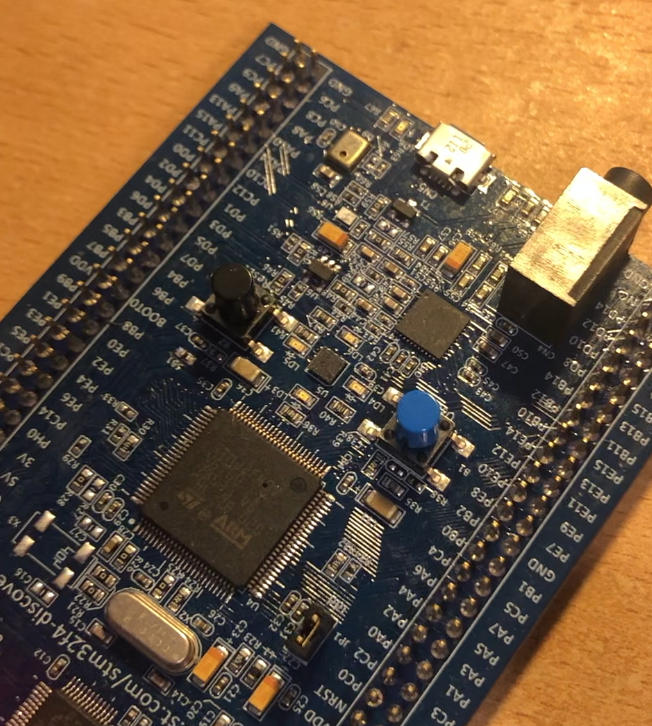
\includegraphics[width=\linewidth]{EventFlagsAus.jpg}
		\caption{suspendierte ISR}
		\label{fig:EventFlagAus}
	\end{subfigure}
	\hspace{1em}
	\begin{subfigure}{.250\textwidth}
		%		\centering
		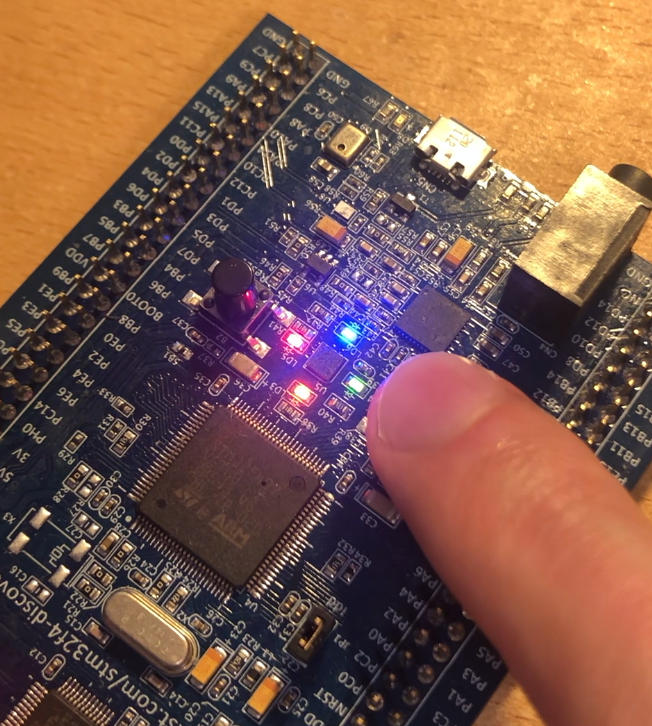
\includegraphics[width=\linewidth]{EventFlagsAn.jpg}
		\caption{aktive ISR}
		\label{fig:EventFlagAn}
	\end{subfigure}
	\caption{Beispiel von Event Flags für Interrupt-Management auf STM32F4 Discovery-Board}
	\label{fig:EventFlagBeispiel}
\end{figure}

Der schematische Ablauf mit Event Flags ist mit Abbildung \ref{fig:ConditionFlag} durchaus vergleichbar, nur dass jetzt Task A durch eine ISR ersetzt wird und eine Eingabe in Form des ausgelösten Ereignisses bekommt bevor das Event Flag gesetzt wird \autocite[vgl.][87]{Cooling2017}. Als weiterführende Lektüre zum Thema Interrupt und Interrupt Service Routine wird \autocite{MikrocontrollerInterrupt} oder weitere Fachliteratur empfohlen. Dabei muss es sich nicht zwingend um ein Hardware-Interrupt handeln, auch andere, benutzerdefinierte Ereignisse können hier verwendet werden. Weiterhin spielt für die hier gewünschten Task-Synchronisierung, also der Zeitraum, in dem der Empfänger - hier Task B - das Event Flag überprüft (\texttt{Check}), eine größere und wichtigere Rolle: Für eine dynamische Reaktion auf ein Ereignis ist ein entsprechend kleines, periodisches Zeitfenster erforderlich. In der in Abbildung \ref{fig:EventFlagBeispiel} dargestellte Demonstration prüft Task B beispielsweise alle 500 Millisekunden ob das zugehörige Event Flag gesetzt ist. Ein weiter mit einer Zwei-Sekunden-Periode durchgeführter Versuch funktionierte ebenfalls, zeigte aber kein flüssiges Verhalten und kann für dieses Szenario ungeeignet sein. Hier muss von Anwendungsfall zu Anwendungsfall verhältnismäßig entschieden werden. Um das Betriebsystem zu entlasten, wird Task B nach jeder negativen Überprüfung bis zur nächsten Periode suspendiert, womit Ressourcen für andere Aufgaben frei werden.\\ 

Die Anwendung der unter \ref{subsec:Koordinierung_mit_Condition_Flags} vorgestellten Techniken zu Condition Flags (z.B. Flag Gruppen) sind auch auf das Konstrukt der Event Flags übertragbar \autocite[vgl.][87-88]{Cooling2017}. Somit ist sowohl eine verbesserte und sicherere Implementierung wie auch für eine größere und ggf. auch verknüpfte Anzahl Event Flags vorhanden.\\

Wie eingangs bereits erwähnt, funktioniert diese Synchronisierung lediglich in eine Richtung: Die Interrupt Service Routine wird durch das vordefinierte Event (z.B. Interrupt) geweckt und setzt das entsprechende Flag, was vom Empfänger-Task im Rahmen seiner regelmäßigen Überprüfung registriert wird. Ist die Überprüfungsperiode entsprechend den Anforderungen gewählt, wird eine mindestens angenäherte Synchronisierung von Ereignis und Reaktion bzw. ISR und Task B erreicht. Sollen zwei oder mehrere Tasks synchronisiert werden, bei der jeder beteiligte Task sowohl Sender als auch Empfänger sein kann, ist eine andere Methodik zu wählen. Diese wird im nächsten Abschnitt vorgestellt.

\subsection{Task-Synchronisation über Signale}
\label{subsec:Task_Synchronisation_Signale}
Mit der bisher vorgestellten Technik, der Event Flags, lässt sich bereits eine Einbahnstraßen-Synchronisation implementieren. Bei einer Problemstellung, bei der etwa mehrere Tasks nach und nach in eine Art Wartestellung gehen (etwa weil ihre Aufgaben erfüllt sind) und alle zu einem gleichen (synchronen) Zeitpunkt erneut starten sollen, hilft dieses Konstrukt allerdings nicht weiter. Hierfür gibt es das Konzept der Signale.\\

Die in Tabelle \ref{tab:Konstrukte} angegebenen Operationen (\texttt{Wait} (warten), \texttt{Send} (senden) und \texttt{Check} (überprüfen)) lassen bereits einen anderen Umgang als bei den bisher vorgestellten Flags erahnen: Eine zentrale Stelle (diese kann sowohl das Betriebssystem selbst bereitstellen oder auch ein eigenes konzipiertes Objekt) übernimmt die Signalverwaltung. Bei ihr registrieren sich die beteiligten Tasks sobald eine der o.g. Operationen ausgeführt wird und diese übernimmt auch die Steuerung des Signals. Damit ist das Signal keinem spezifischem Task zugeordnet und auch keine von diesem ausgehende Synchronisierung \autocite[vgl.][91]{Cooling2017} Abbildung \ref{fig:Signale_gesamt} stellt die drei auftretenden Möglichkeiten vor.

\begin{figure}[h]
	\centering
	\fbox{
	\begin{subfigure}[t]{.353\columnwidth} % Werte mal so eingestellt lassen! .353
		\def\svgwidth{\columnwidth} % Breite wird auf Blattbreite (spalte) gesetzt
		\input{Signale_a.pdf_tex}
		\caption{\label{subfig:Signale_a}}
	\end{subfigure}
}\fbox{
	\begin{subfigure}[t]{.35\columnwidth} % Werte mal so eingestellt lassen! .35
		\def\svgwidth{\columnwidth}
		\input{Signale_b.pdf_tex}
		\caption{\label{subfig:Signale_b}}
	\end{subfigure}
}\fbox{
	\begin{subfigure}[t]{.1735\columnwidth} % Werte mal so eingestellt lassen! .1735
		\def\svgwidth{\columnwidth}
		\input{Signale_c.pdf_tex}
		\caption{\label{subfig:Signale_c}}
	\end{subfigure}
}
	\begin{subfigure}{.40\columnwidth} % Werte mal so eingestellt lassen! .40
		\def\svgwidth{\columnwidth}
		\input{Signale_Legende.pdf_tex}
	\end{subfigure}
	\caption{\label{fig:Signale_gesamt}Task-Synchronisation mittels Signalen \autocite[vgl.][90]{Cooling2017}}
\end{figure}

Zunächst sollen in den Abbildungen \ref{subfig:Signale_a} und \ref{subfig:Signale_b} zwei Tasks synchronisiert werden. Beide Darstellungen unterscheiden sich lediglich in der Reihenfolge, welche Operation zuerst auf ein Signal gewirkt wird: Der Task, welcher sich zuerst mit einer Operation meldet, wird suspendiert bis er - zusammen mit dem anderen Task - das synchronisierte Signal zur Wiederaufnahme erhält. Beide starten dann synchron zum gleichen Zeitpunkt \autocite[vgl.][90-91]{Cooling2017}.
Der sichtbare zeitliche Abstand bevor beide Tasks erneut starten, nachdem sie zur Synchronisierung gemeldet sind, kann darin begründet sein, dass zuerst ein Zeitfenster abgewartet werden soll oder ein Jitter (unvorhersehbare Verzögerung) auftritt, der den Start verzögert.
Option \ref{subfig:Signale_c} zeigt, wie ein einzelner Task synchronisiert wird, ohne bekanntes Mitspiel anderer Tasks: Eine Überprüfung des Signalstatus erfolgt und ggf. eine Suspendierung oder eine sofortige Wiederaufnahme. Hierbei kann die Signalverwaltung (Exekutive) auch eine interne Logik besitzen und zum Timing verschiedener einzelner oder mehrerer Tasks benutzt werden \autocite[vgl.][91]{Cooling2017}.\\

Die Umsetzung von Signalen erfolgt normalerweise über Funktionen \autocite[vgl.][91]{Cooling2017}, wie im folgenden mit C beispielhaft skizziert:
\begin{lstlisting}[language=C]
/* Sendet das Signal */
void Send(SyncSignal SignalName);

/* Warte-Anfrage auf Signal */
void Wait(SyncSignal SignalName);

/* Prueft ob ein Task wartet */
typedef enum {false, true} bool; // Def. fuer C hilfreich
bool Check(SyncSignal SignalName);
\end{lstlisting}
Zusammengefasst ist dabei folgendes, aus Abbildung \ref{fig:Signale_gesamt} abgeleitetes Verhalten in den Funktionen zu implementieren um Signale vollständig umzusetzen:
\begin{itemize}
	\item \texttt{Send}: Sendender Task wird suspendiert sofern kein anderer Task bereits eine \texttt{Wait}-Anfrage gestellt hat.
	\item \texttt{Wait}: Wird das Signal nicht bereits gesendet, wenn diese Anfrage gestellt wird, wird der Task suspendiert. Andererseits wird der sendende Task reaktiviert und beide Tasks werden synchron wieder ausgeführt.
	\item \texttt{Check}: Gibt $true$ zurück, wenn das Signal gesendet wird, ansonsten $false$.
\end{itemize}
Somit sind Signale eine gute Methode, um in zwei oder mehrere Richtungen zu synchronisieren, da hier jeder Task sowohl Sender als auch Empfänger des Synchronisationsprozesses sein kann. Diese Technik wird aber von eher wenigen Echtzeitbetriebssystemen als native Implementierung angeboten \autocite[vgl.][91]{Cooling2017}.

\section{Datentransfer ohne Synchronisation oder Koordination}
\label{sub:Datentransfer_ohne_Sync_Koord}
Ist ein Datenaustausch zwischen Tasks erforderlich (zum Beispiel weil Daten zur Weiterverarbeitung benötigt werden), die aber nicht zur Koordination verwendet und ebenfalls nicht an zeitliche Kriterien gebunden sind, wird dies über verschiedene Datenverarbeitungsmechanismen bewerkstelligt. Diese lassen sich primär in zwei Kategorien unterteilen. Durch die fehlenden scharfen Kriterien einer Synchronisation oder Koordination, sind sie unkomplizierter in der Benutzung und leichter zu implementieren.
\begin{figure}
	\centering
	%\def\svgwidth{\columnwidth} % Breite wird auf Blattbreite (spalte) gesetzt
	\begin{subfigure}[b]{.450\textwidth}
		\def\svgwidth{\columnwidth}
		\input{RandomAccess.pdf_tex}
		\caption{\label{subfig:zufaelliger_Zugriff}}
	\end{subfigure}
	\hspace{3em}
	\begin{subfigure}[b]{.450\textwidth}
		\def\svgwidth{\columnwidth}
		\input{SequentialAccess.pdf_tex}
		\caption{\label{subfig:sequentiell_Zugriff}}
	\end{subfigure}
	\caption{\label{fig:Datentransfer_Ueberblick}Datentransfer zwischen Tasks \autocite[vgl.][95]{Cooling2017}}
\end{figure}

Abbildung \ref{fig:Datentransfer_Ueberblick} zeigt die Unterscheidung der hier aufgeführten zwei Prinzipien \glqq zufälliger Zugriff \grqq \ref{subfig:zufaelliger_Zugriff} und \glqq sequentieller Zugriff \grqq \ref{subfig:sequentiell_Zugriff}. Während bei ersterem eine Vielzahl an Tasks die gleiche Datenstruktur verwenden können, erfolgt bei zweiterem eine Eins-zu-eins-Weiterleitung (von Task zu Task). Damit besitzt jeder Datentyp auch seine Daseinsberechtigung und wird im folgenden genauer vorgestellt.
\subsection{Pools}
\label{subsec:Pools}
Pools sind per Definition ein Read-Write Random Access Data Store \autocite[vgl.][94]{Cooling2017}. Das bedeutet: Ein Pool besitzt eine variable Größe, ist also theoretisch nicht auf eine bestimmte, feste Anzahl an möglichen beinhalteten Elementen beschränkt, kann aber nur vordefinierte Objekte speichern (die stets die gleiche Speichergröße besitzen). Folgende Codedarstellung soll dieses Prinzip in C++ verdeutlichen:
\begin{lstlisting}[language=C++]
struct Data {
	char* id;
	int value;
};

Pool<Data> fifoList;
\end{lstlisting}
Ein Typ $Data$ wird deklariert, welcher einen $char$-Zeiger sowie einen Integer enthält. Der Pool $fifoList$ kann nur Objekte dieses Typs aufnehmen und verwalten. Wie noch gezeigt wird, bieten Pools allerdings - abhängig von der Implementierung - den Vorteil, dass sie nicht in einem zusammenhängenden Speicherblock untergebracht sein müssen, sondern die Daten im Speicher verteilt liegen können. Hier sei noch angemerkt, dass das Objekt, welches vom $char$-Zeiger referenziert wird, nicht im Speicherbereich des Pools liegen muss und in einem anderen Teil des Speichers liegen kann.

Eine weitere Eigenschaft eines Pools ist damit die (Daten-)Kapselung: Außerhalb existierender Code bzw. Tasks erhalten lediglich Zugriff auf die Lese- und Schreib-Methoden des Pools, haben aber keinerlei Einfluss auf die interne Organisation der Daten oder Informationen über den Speicherort dieser und können auch nicht ohne direkte Kommunikation mit öffentlichen Methoden des Pools lesen oder schreiben.\\

\begin{figure}%{.250\textwidth}
	\centering
	\def\svgwidth{.50\columnwidth}

	\input{Pool.pdf_tex}
	\caption{\label{fig:Pool}Ein mit Mutex geschützter Pool \autocite[vgl.][95]{Cooling2017}}
\end{figure}

Diese Kapselung soll in Abbildung \ref{fig:Pool} dargestellt werden, sie zeigt außerdem den schematischen Aufbau dieses Datentyps: Über eine Schnittstelle (Interface), die mindestens die o.g. (R/W) Methoden bereitstellt, erfolgt die Kommunikation bzw. die Datenübermittlung in beide Richtungen. Um Schreib- oder Lesefehler zu vermeiden, verwenden Pools intern gern einen sogenannten Mutex, also einen Sicherungsmechanismus, der keinen mehrfach Zugriff auf Daten erlaubt. Tasks die während eines gerade stattfindenden Zugriffs ebenfalls Daten erlangen möchten, werden suspendiert und erhalten nach der internen Freigabe durch den Mutex nacheinander anschließend Zugriff auf die Daten. Dies ist vergleichbar mit einer Schrankenabfertigung im Straßenverkehr \autocite[vgl.][95]{Cooling2017}.\\

Allgemein bekannte Datenstrukturen die sich Pools zuzuordnen lassen, sind etwa FIFO (\textbf{F}irst \textbf{I}n \textbf{F}irst \textbf{O}ut) und LIFO (\textbf{L}ast \textbf{I}n \textbf{F}irst \textbf{O}ut) Listen (basierend auf verkettete Listen) sowie Heaps in verschiedenen Ausführungen. Gerade verkettete Listen bieten den bereits erwähnten Vorteil, dass ein Pool nicht auf einem zusammenhängenden Speicherblock liegen muss, sondern die einzelnen Listenelemente, durch Zeiger miteinander verbunden, im Speicher verteilt liegen können. Das macht Pools zu einer für das Speichermanagement flexibleren Datenstruktur \autocite[vgl.][96]{Cooling2017}.

\subsection{Warteschlangen}
\ref{subsec:Warteschlange}
Warteschlangen (Queues) eigenen sich ebenfalls für die Datenübertragung zwischen Tasks, unterscheiden sich - bezogen auf diesen Anwendungsbereich - aber in diversen Punkten von den bereits vorgestellten Pools. Zunächst besitzen Warteschlangen in diesem Kontext eine feste Größe: Sobald sie im Code deklariert werden, sind sie in ihrer Größe bzw. in der Anzahl Elemente, die sie aufnehmen können, nicht mehr veränderbar. Hier muss eine vernünftige Größe gewählt werden, da schließlich nicht unendlich viel Speicher zur Verfügung steht. Des weiteren sind sie am ehesten für die Task-zu-Task-Datenübertragung konzipiert und bildlich vergleichbar mit einem Einbahnstraßen-Verbindungstunnel: Ein Task legt Daten in der Warteschlange ab, ein anderer liest diese daraus (\ref{subfig:sequentiell_Zugriff}). Damit ergeben sich die beiden Funktionen \texttt{Dequeue} und \texttt{Enqueue}, die entweder ein Objekt aus der Warteschlange zurückgeben oder ihr ein neues hinzufügen. Abbildung \ref{subfig:sequentialAccess} verdeutlicht diese Funktionsweise einer Warteschlange.\\

Intern werden - neben einem $n$-großen Feld (Array) - gekapselt zwei Indizes (in Form von vorzeichenlosen Integern oder Zeigern) gespeichert, die zwei wichtige Punkte innerhalb der (FIFO-)Warteschlange markieren: Das Feld, an dem das nächste Element eingefügt wird und das Feld, des Objekts, das als nächstes entnommen wird (im Falle einer FIFO-Struktur gleich dem ältesten Element). Außerdem wird ein Zähler gespeichert, der Auskunft über die Anzahl Elemente in der Warteschlange gibt.

\begin{figure}
	\centering
	\def\svgwidth{0.30\columnwidth}
	\input{RingBuffer_a.pdf_tex}
	\caption{\label{fig:RingBuffer}Prinzip einer FIFO-Warteschlange als Ring Buffer dargestellt \autocite[vgl.][97]{Cooling2017}}
\end{figure}

Die Implementierung einer Warteschlange kann auf verschiedene Arten erfolgen, hier wird beispielhaft die Implementierung als Ring Buffer (auch Circular Buffer) aufgezeigt: Zur Initialisierung zeigen beide Zeiger bzw. Indizes auf das erste Feld des internen Arrays. Der Zähler wird auf Null gesetzt. Mit diesen Informationen gilt es zwei Fälle im Betrieb gesondert zu behandeln, nämlich dann, wenn beide Zeiger/Indizes auf das gleiche Feld zeigen:
\begin{itemize}
	\item Ist der Zähler bei $0$ (die Warteschlange also leer), darf kein weiteres Element mehr entnommen werden können.
	\item Ist der Zähler größer $0$ (die Warteschlange somit vollständig befüllt) wird bei \texttt{Enqueue} das älteste Element im Falle eines Hinzufügens überschrieben.
\end{itemize}
In jedem anderen Fall von \texttt{Enqueue} werden alle in der Warteschlange befindlichen Elemente um ein Feld nach hinten verschoben (damit wird das älteste Element überschrieben) und das neuste Element wird vorne eingefügt.

\texttt{Dequeue} übergibt stets das älteste Element und entnimmt es gleichzeitig der Warteschlange, womit ein leeres Feld entsteht und der betreffende Zeiger bzw. Index so angepasst wird, dass er auf das zweitälteste Element zeigt.\\

Damit entsteht eine relativ einfach zu implementierende Datenstruktur für die Task-zu-Task-Kommunikation mit der verschiedene Auslieferungskriterien (FIFO/LIFO) leicht umgesetzt werden können.

\section{Task-Synchronisation mit Datentransfer}
\label{sub:Task_Synchronisation_Datentransfer}
Daten, die mit einer zeitlichen Priorität zwischen Tasks ausgetauscht werden müssen, also genau zum richtigen Zeitpunkt (oder schnellstmöglich) beim Empfänger bereit stehen müssen, werden ebenfalls mit einer Datenstruktur transferiert. An diese besteht jedoch ein höherer Anspruch, da sie die Synchronisation sicherstellen und auch Daten verwalten muss. Die Daten müssen also in einem vordefinierten Zeitfenster beim Empfänger eingehen. Dies kann so gehandhabt werden, als das die Daten schnellstmöglich beim Empfänger-Task verfügbar sein müssen. Dies ist die höchste Kunst der Datenübermittlung zwischen Tasks und eine Kerneigenschaft von Echtzeitbetriebssystemen. Die für diese Aufgabe zugedachte Datenstruktur heißt Mailbox. Sie kann auf verschiedene Arten funktionieren, welche nun aufgezeigt werden.

\subsection{Mailbox}
Für die synchronisierte Datenübermittlung in Echtzeitbetriebssystemen gibt es einige Datenstrukturen, die unter dem Begriff Mailbox zusammengefasst werden. Eine Mailbox kann mit folgenden beiden Befehlen implementiert werden:
\texttt{Post} und \texttt{Pend}. Die Schemata \ref{subfig:Mailbox_a} und \ref{subfig:Mailbox_b} ähneln nicht zufällig denen aus Kapitel \ref{subsec:Task_Synchronisation_Signale} (Signale). Im Grunde lässt sich eine Mailbox bereits mithilfe einer Datenstruktur, wie sie in Kapitel \ref{sub:Datentransfer_ohne_Sync_Koord} vorgestellt wurden und einem Signal vollständig nachbilden.

Demzufolge sind die Kommandos einer Mailbox in diesem Fall auch von denen der Signale abgeleitet: \texttt{Post} bedeutet hier, dass eine Benachrichtigung an die Mailbox geschickt wird, die von einem anderen Task entgegengenommen werden kann. Diese Aufnahmebereitschaft zeigt der Empfänger-Task mit dem Kommando \texttt{Pend} an (ähnlich zu \texttt{Wait}). Hat sich der Empfänger-Task noch nicht bei der Mailbox zur Abholung bereit gemeldet, wird der Sender suspendiert. Auch umgekehrt ist der Fall möglich, wie Abbildung \ref{subfig:Mailbox_b} zeigt: Hier wird zuerst nach einer Nachricht gefragt und bis diese vorliegt, wird der entsprechende Task suspendiert. Besteht letztendlich eine Verbindung zweier Tasks über die Mailbox, wird die betreffende Nachricht ausgetauscht.
\begin{figure}[h]
	\centering
	\fbox{
		\begin{subfigure}[t]{.36\columnwidth} % Werte mal so eingestellt lassen! .39
			\def\svgwidth{\columnwidth} % Breite wird auf Blattbreite (spalte) gesetzt
			\input{Mailbox_c.pdf_tex}
			\caption{\label{subfig:Mailbox_a}}
		\end{subfigure}
	}\fbox{
		\begin{subfigure}[t]{.3530\columnwidth} % Werte mal so eingestellt lassen! .387
			\def\svgwidth{\columnwidth}
			\input{Mailbox_d.pdf_tex}
			\caption{\label{subfig:Mailbox_b}}
		\end{subfigure}
	}\fbox{
		\begin{subfigure}[t]{.1485\columnwidth} % Werte mal so eingestellt lassen! .1918
			\def\svgwidth{\columnwidth}
			\input{Mailbox_b.pdf_tex}
			\caption{\label{subfig:Mailbox_c}}
		\end{subfigure}
	}
	\begin{subfigure}{.40\columnwidth} % Werte mal so eingestellt lassen! .40
		\def\svgwidth{\columnwidth}
		\input{Signale_Legende.pdf_tex}
	\end{subfigure}
	\caption{\label{fig:Mailbox_gesamt}Datentransfer mit Task-Synchronisation \autocite[vgl.][99]{Cooling2017}}
\end{figure}
Abbildung \ref{subfig:Mailbox_c} zeigt eine andere Herangehensweise zur synchronen Datenübermittlung: Während bei \ref{subfig:Mailbox_a} und \ref{subfig:Mailbox_b} eine synchrone Übermittlung das Ziel ist, soll hier eine schnellstmögliche Datenübermittlung erreicht werden. Diese wird in vielen Echtzeitbetriebssystemen als Publisher/Subscriber-Prinzip umgesetzt: Eine öffentliche Datenstruktur, etwa ein sogenanntes Topic, vergleichbar mit einem Kanal, wird eingerichtet. In dieses Topic können Tasks Daten schreiben (publishen). Genauso können andere Tasks diese Datenstruktur abonnieren (subscriben) und erhalten bei neu hinzugefügten Daten eine Benachrichtigung. Dies kann z.B. als Ereignis umgesetzt werden (indem eine vordefinierte Funktion aufgerufen wird). Damit liegt keine direkte Verbindung der Tasks vor, sondern es werden nur Benachrichtigungen über die Datenstruktur selbst ausgetauscht.\\

Tabelle \ref{tab:SyncDaten} zeigt die Teilergebnisse einer Messung, die auf einem Echtzeitbetriebssystem mit dem Publisher/Subscriber-Prinzip durchgeführt wurde: Alle fünf Sekunden beginnend ab $10 s$ der Laufzeit des Systems wird - zum Vergleich - die aktuelle Systemzeit ausgegeben und jede neue Sekunde die aktualisierte Systemzeit in ein Topic (Mailbox) veröffentlicht. Der Empfänger erhält diese Zeitangabe (in Form von Nanosekunden seit Systemstart) und gibt die Differenz zur aktuellen Systemzeit aus, womit die Dauer sichtbar wird, wie lange die Daten vom Sender zum Empfänger unterwegs waren. Durchgeführt wurde diese Messung auf Basis einer virtuellen Maschine und dem Echtzeitbetriebssystem RODOS \autocite{Wuerzburg2019}.

\begin{table}[h]
	\centering % Tabelle zentrieren
	\def\arraystretch{1.2} % Vertikales Padding
	\setlength{\tabcolsep}{0.5em} % Horizontales Padding
	\begin{tabular}[h]{|lrl|}
		\hline
		0: & 10.000.003.014 & ns ($t_{System}\approx 10 s$) \\
		1: & 1.206 & ns \\
		2: & 686 & ns \\
		3: & 691 & ns \\
		4: & 736 & ns \\
		5: & 757 & ns \\
		6: & 15.000.003.484 & ns ($t_{System}\approx 15 s$) \\
		7: & 762 & ns \\
		8: & 724 & ns \\
		9: & 769 & ns \\
		10: & 690 & ns \\
		11: & 633 & ns \\
		12: & 20.000.002.990 & ns ($t_{System}\approx 20 s$) \\
		\hline
	\end{tabular}%}
	\caption{\label{tab:SyncDaten} Zeitliche Messung der Dauer eines synchronisierten Datentransfers}
\end{table}
Diese Messung soll zugleich einen Eindruck vermitteln, in welcher zeitlichen Größenordnung die Datenübermittlung in etwa erfolgt. Es ist leicht erkennbar, dass sich die Zeitdifferenz, mit einer Ausnahme, im Nanosekundenbereich bewegt. Für viele Anwendungsbereiche dürfte dieser Jitter noch im vertretbaren Bereich liegen.\\

Mit den in der Abbildung \ref{fig:Mailbox_gesamt} dargestellten Möglichkeiten, können so relativ leicht Daten synchron zwischen Tasks ausgetauscht werden. Entweder über eine Mailbox die auf Signalen basiert oder mittels des Publisher/Subscriber-Prinzips.

\section{Zusammenfassung}
Task-Kommunikation ist ein unabdingbares Instrument in Echtzeitbetriebssystemen und in beinahe jeder Anwendung auf diesem Gebiet erforderlich. Es wurde abhängig der Fälle aufgezeigt welche Art der Kommunikation am besten ist und wie diese bestmöglich umgesetzt wird.\\

So erreicht man Task-Koordination, die Steuerung eines Ablaufs, am besten mit Condition Flags, eine einseitige-Synchronisierung mit Event Flags und kann beiderseits Synchronisierung über Signale umsetzen. Weiterhin wurden verschiedene Möglichkeiten gezeigt, wie diese Methoden implementiert werden können - abhängig von der erforderlichen Entwicklungsstrategie.\\

Auch, Daten von einem Task zu einem anderen (oder mehreren) zu übermitteln bzw. zu transferieren ist eine wichtige Aufgabe und kann wahlweise mit der Datenstruktur eines Pools oder eine Warteschlange bewerkstelligt werden. Viele Echtzeitbetriebssysteme bieten von Haus aus entsprechende Typen an, wobei eine eigene Implementierung aufgrund der fehlenden Komplexität nicht allzu schwierig ist.\\

Die Königsdisziplin, eine synchronisierte Datenübertragung zwischen zwei Tasks erfolgt über das Konstrukt der Mailbox und ist in vielen Echtzeitbetriebssystemen als Publisher/Subscriber-Prinzip umgesetzt, welches den Empfänger automatisch bei Eintreffen neuer Daten benachrichtigt, sodass diese schnellstmöglich weiterverarbeitet werden können.\\

Mit dem in dieser Arbeit vorgestelltem Handwerkszeug ist das Thema der Intertask-Kommunikation in Echtzeitbetriebssystemen übersichtlich zusammengefasst und jedes größere Anwendungsszenario abgedeckt.

\printbibliography


\end{document}